\section{4. úkol}
\subsection*{Zadání}
Najděte a nakreslete definiční obor funkce 
\begin{eqnarray}f(x,y) = \dfrac{1}{\mathrm{ln}(\mathrm{cos}(\pi x) - y)} + \sqrt{\mathrm{cos}(\pi y) + x}
\label{eq:def}
\end{eqnarray}
\subsection*{Rozbor příkladu}
Máme najít definiční obor funkce dvou neznámých, která je zadána přepisem \ref{eq:def}. 

Najdeme tedy definiční obory všech elementárních funkcí a výsledný definiční obor bude průnikem těchto dílčích definičních oborů.

\subsection*{Řešení}
Musí jednoznačně platit, že
\begin{displaymath}
\mbox{cos}(\pi x) - y  > 0 \quad \wedge \quad \mbox{cos}(\pi x) - y \neq 1 \quad \wedge \quad \mbox{cos}(\pi y) + x \geq 0
\end{displaymath}

\noindent Nerovnice je možné si nyní zakreslit

\begin{figure}[h]
  \centering
  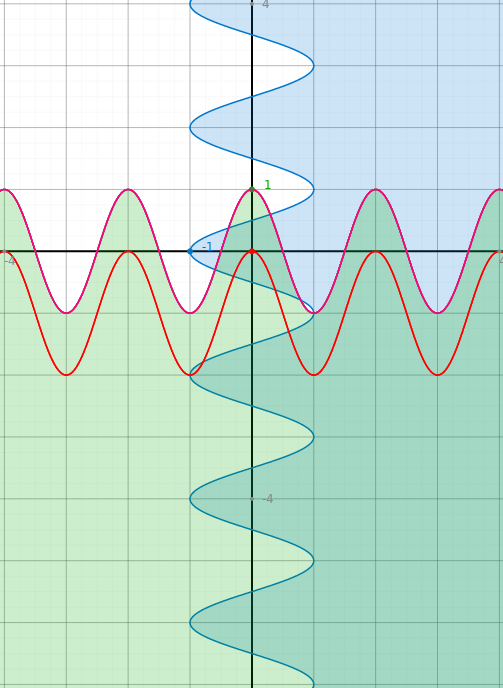
\includegraphics[width=8cm]{assets/grafKomplet.png}
  \caption{Červená a růžová barva do průniku nepatří, modrá a zelená ano}
\end{figure}
